\documentclass[11pt]{article}


    \usepackage[breakable]{tcolorbox}
    \tcbset{nobeforeafter} % prevents tcolorboxes being placing in paragraphs
    \usepackage{float}
    \floatplacement{figure}{H} % forces figures to be placed at the correct location
    \usepackage{multicol}
	\usepackage[english]{babel}
    \usepackage{tabularx}
    \usepackage{subfigure}
    \usepackage{picture}
    \usepackage{amsmath}
    \usepackage{hyperref}
    \hypersetup{
    colorlinks=true,
    linkcolor=blue,
    filecolor=magenta,      
    urlcolor=cyan,
    }
    \usepackage{graphicx}    
    \usepackage{caption}
    \usepackage{adjustbox} % Used to constrain images to a maximum size 
    \usepackage{xcolor} % Allow colors to be defined
    \usepackage{enumerate} % Needed for markdown enumerations to work
    \usepackage{geometry} % Used to adjust the document margins
    \usepackage{amsmath} % Equations
    \usepackage{amssymb} % Equations
    \definecolor{urlcolor}{rgb}{0,.145,.698}
    \definecolor{linkcolor}{rgb}{.71,0.21,0.01}
    \definecolor{citecolor}{rgb}{.12,.54,.11}
    

    
    % Prevent overflowing lines due to hard-to-break entities
    \sloppy 
    % Setup hyperref package
    \hypersetup{
      breaklinks=true,  % so long urls are correctly broken across lines
      colorlinks=true,
      urlcolor=urlcolor,
      linkcolor=linkcolor,
      citecolor=citecolor,
      }
    % Slightly bigger margins than the latex defaults
    
    \geometry{verbose,tmargin=1in,bmargin=1in,lmargin=0.4in,rmargin=1in}
    \usepackage{fancyhdr}
    \pagestyle{fancy}
    \renewcommand{\footrulewidth}{1pt}
    \rhead{e11921655 Fabian Holzberger \\ e01526208 Jan Ellmenreich}
    \lhead{VU\,184.725\\ High Performance Computing}
    \cfoot{\thepage}
    \setcounter{secnumdepth}{0}
    \setlength\parindent{0pt}

    \usepackage{booktabs}

    \usepackage{listings}
    \usepackage[linesnumbered,ruled,vlined]{algorithm2e}
    \newcommand\mycommfont[1]{\footnotesize\ttfamily\textcolor{blue}{#1}}
    \SetCommentSty{mycommfont}
    \SetKwInput{KwInput}{Input}                % Set the Input
    \SetKwInput{KwOutput}{Output}              % set the Output



\title{Exercise0 Dataset description}
\author{e De Ronde Maria \\ e Andre Quentin  \\ e11921655 Fabian Holzberger }
\date{\today}

\begin{document}
\graphicspath{{./figures/}}
\maketitle
\section{Classification Dataset: Email-Spam}
We have chosen a Emai-Spam Dataset for classification (\href{https://www.kaggle.com/nitishabharathi/email-spam-dataset?select=enronSpamSubset.csv}{link to dataset}). The goal for this dataset is to distinguish by a machine learning algorithm between  spam and non-spam emails. The datasets are given in \texttt{csv} format and the structure is shown in table~\ref{tab::0}. Here we see that the dataset has a Body-column that contains the text-body of an email and a Label-column that is either set to 1 for spam E-mails or 0 for non-spam E-mails. 

\begin{figure}[h]
  \begin{tabular}{ | c | p{13cm} | c |}
    \hline
    Index & Body & Label \\
    \hline
    100 & 
    Subject: inexpensive online medication here
 pummel wah springtail cutler bodyguard
 we ship quality medications overnight to your door !...
    & 1 \\ \hline
    6006
    &
    Subject: organizational changes
 we are pleased to announce the following organizational changes :
 enron global assets and services
 in order to increase senior management focus on our international businesses... 
    & 0 \\
    \hline
    \end{tabular}
    \caption{Structure of the Email-Spam Dataset}
    \label{tab::0}
  \end{figure}

The dataset contains in total 10.000 samples where 50\% of the samples are spam- and 50\% are non-spam E-mails. Since there are no missing values the dataset is perfectly balanced with respect to the target attribute. We aim to apply the \textbf{Bag of Words} method to the dataset. This Method extracts the $N$ most common Words from all E-mails and then maps an E-mail to a vector $v$ such that the component $m$ of $v$ is an nonegative integer that counts the occureces of the $m$th most common word in the corresponding E-mail. From that we conclude that the dimension of our dataset is $N+1$ since we also include the target attribute.  Note that we apply the following cleanup steps to all Emails to remove data that we expect to not improve the classification: 1. remove links, 2. remove characters except alphabetical ones, 3.convert uppercase-chars into lowercase-chars, 3. lemmatize words 4. remove stopwords. By that we reduce the number of total different words in all e-mails from 86733 words to 74618 words by the cleanup step. This also illustrates that our classification algorithm has to work with data that is hight dimensional (dimension much larger than 1000).          
In figure~\ref{fig::word-counts} we show the most common words in spam and non-spam emails.  


\begin{figure}[H]
\begin{picture}(400,220)
\put(-40,0){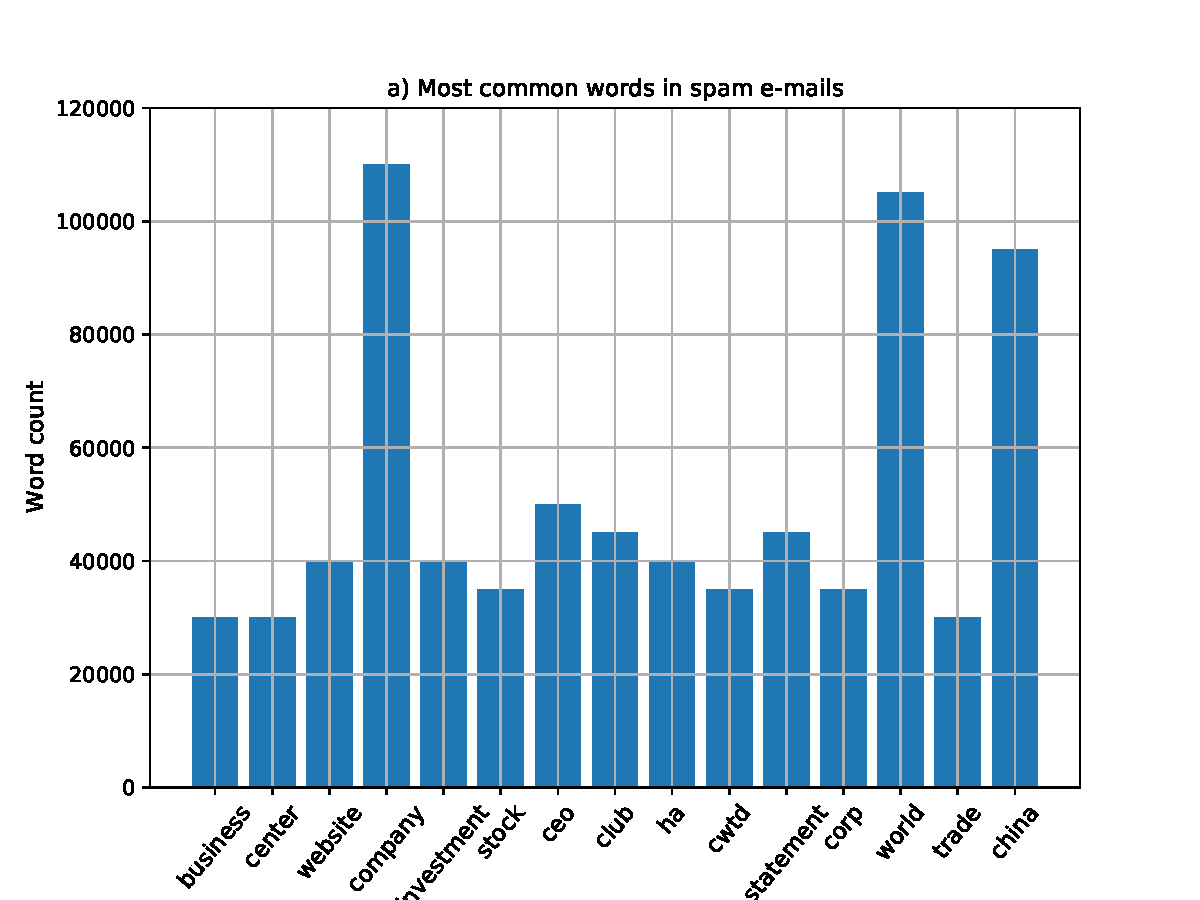
\includegraphics[width=0.55\linewidth]{spam_count.pdf}}
\put(240,0){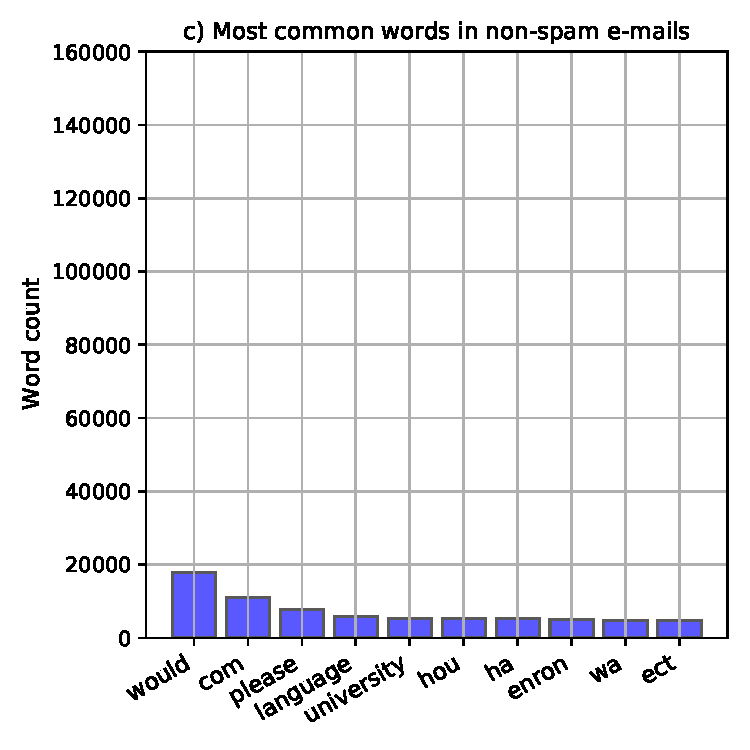
\includegraphics[width=0.55\linewidth]{ham_count.pdf}}
%\put(95,190){\textit{a})}
%\put(375,190){\textit{b})}
\end{picture}
  \caption{Figure \textit{a})15  most common words in spam e-mails \textit{b})15 most common words in non-spam e-mails}
\label{fig::word counts}
\end{figure}



%Bibliography
\newpage
\bibliographystyle{plain}
\bibliography{Biblothek}



\end{document}
